\chapter{Аналитический раздел}
В данном разделе будет рассмотрено описание работы классического алгоритма умножения матриц и алгоритма умножения матриц Винограда.

\section{Основные сведения об алгоримтах}
Умножение матриц - одна из основных операций над матрицами. В результате данной операции мы получаем новую матрицу. Данная операция становится возможна только в том случае, если число столбцов в первом сомножителе равно числу строк во втором. При выполнении этого условия говорится, что матрицы согласованы. Из данного условия следует, что произведение матриц некоммутативно.

\section{Классический алгоритм}
Пусть даны две прямоугольные матрицы A и B, размерности $n\times m$ и $m\times k$ соответственно:

\begin{equation}
  A_{n\times m} =
  \left[ {\begin{array}{cccc}
    a_{11} & a_{12} & \cdots & a_{1m}\\
    a_{21} & a_{22} & \cdots & a_{2m}\\
    \vdots & \vdots & \ddots & \vdots\\
    a_{n1} & a_{n2} & \cdots & a_{nm}\\
  \end{array} } \right]
\label{mat_a}
\end{equation}

\begin{equation}
  B_{m\times k} =
  \left[ {\begin{array}{cccc}
    a_{11} & a_{12} & \cdots & a_{1k}\\
    a_{21} & a_{22} & \cdots & a_{2k}\\
    \vdots & \vdots & \ddots & \vdots\\
    a_{m1} & a_{m2} & \cdots & a_{mk}\\
  \end{array} } \right]
\label{mat_b}
\end{equation}

Тогда произведением матриц А, В будет является матрица C размерностью $n \times k$:

\begin{equation}
  C_{n\times k} =
  \left[ {\begin{array}{cccc}
    a_{11} & a_{12} & \cdots & a_{1k}\\
    a_{21} & a_{22} & \cdots & a_{2k}\\
    \vdots & \vdots & \ddots & \vdots\\
    a_{n1} & a_{n2} & \cdots & a_{nk}\\
  \end{array} } \right]
\label{mat_c}
\end{equation}

где:

\begin{equation}
C_{ij} = \sum_{l=1} ^{m} a_{il} b_{lj} (i = \overline{1,n}, j = \overline{1,k})
\label{c_elem}
\end{equation}

Стандартный алгоритм умножения матриц использует эту формулу.

\section{Алгоритм Винограда}

При рассмотрении операции умножения матриц, можно сделать вывод, что каждый элемент в матрице C на самом деле является скалярным произведением векторов строки из матрицы A и столбца из матрицы B. При помощи предварительной обработки мы можем выполнить часть работы заранее, что позволит снизить количество операций.

Рассмотрим два вектора V и W:
\begin{equation}
V = (\upsilon_{1}, \upsilon_{2}, \upsilon_{3}, \upsilon_{4})
\label{v_vec}
\end{equation}

\begin{equation}
W = (\omega_{1}, \omega_{2}, \omega_{3}, \omega_{4})
\label{w_vec}
\end{equation}

Тогда скалярное произведение этих векторов может быть записано следующим образом.
\begin{equation}
V \times W = \upsilon_{1}\omega_{1} + \upsilon_{2}\omega_{2} + \upsilon_{3}\omega_{3} + \upsilon_{4}\omega_{4}
\label{vw_vec}
\end{equation}

Это равенство может быть преобразовано следующим образом:
\begin{equation}
V \times W = (\upsilon_{1} + \omega_{2})(\upsilon_{2} + \omega_{1}) + (\upsilon_{3} + \omega_{4})(\upsilon_{4} + \omega_{3}) - \upsilon_{1}\upsilon_{2} - \upsilon_{3}\upsilon_{4} + \omega_{1}\omega_{2} + \omega_{3}\omega_{4}
\label{vw_vec_rest}
\end{equation}

Данное выражение позволяет сэкономить количество операций при вычислении благодаря тому, что правую часть можно вычислить заранее отдельно для каждой матрицы и использовать уже посчитанный результат при вычислении. При выполнении программы над предварительно обработанными элементами выполняются только первые два умножения и последующие пять сложений, а таже два сложения в скобках. Так как сложение быстрее умножения, алгоритм должен работать быстрее стандартного.

\section{Модель вычислений}
Для того, чтобы вычислить трудоёмкость алгоритма, введём следующую модель вычислений:

\begin{enumerate}
	\item операторы, трудоёмкость которых равна 1: +, -, /, \%, ==, !=, <, >, >=, <=, [], ++;
	\item трудоёмкость оператора выбора if (условие) then A else B рассчитывается как $f_{\text{условия}} + f_{A}$ или $f_{B}$ в зависимости то того, какое условие выполняется;
	\item трудоёмкость цикла рассчитывается как $f_{for} = f_{\text{инициализации}} + f_{\text{сравнения}} + N(f_{\text{тела}} + f_{\text{инициализации}} + f_{\text{сравнения}})$;
	\item трудоёмкость вызова функции равна 0.
\end{enumerate}

\section{Вывод}
В данном разделе были рассмотрены основные теоретические сведения о классическом алгоритме умножения матриц и об алгоритме Винограда умножения матриц. В результате чего был сделаны выводы о том, что на вход алгоритмов подаются матрицы и их размерности, а на выходе возвращается матрица с результатом. Алгоритмы работают на матрицах с согласованными размерностями от 0 до физически возмого предела для изпользуемой машины. В качестве критерием для сравнения будет использоваться время работы алгоритмов. Также был проведён анализ модели вычислений, которая будет использоваться для вычисления трудоёмкости алгоритмов.

\chapter{Конструкторский раздел}

В данном разделе будут рассмотрены схемы, структуры данных, способы тестирования, описания памяти для следующих алгоритмов:
\begin{enumerate}
	\item классический алгоритм умножения матриц;
	\item алгоритм Винограда для умножения матриц;
	\item оптимизированный алгоритм Винограда для умножения матриц.
\end{enumerate}

\section{Тестирование алгоритмов}

Описание классов эквивалентности:
\begin{enumerate}
	\item проверка на общем случае матриц;
	\item проверка на векторах (частный случай матрицы);
	\item проверка на единичной матрице;
	\item проверка на нулевой матрице.
\end{enumerate}

Описание тестов:
\begin{enumerate}
	\item тест на двух матрицах размером n x k и k x m, где n > 0, k >  0, m > 0;
	\item тест на двух матрицах размером n x k и k x m, где n = 1, k >  0, m > 0;
	\item тест на двух матрицах размером n x k и k x m, где n > 0, k >  0, m = 1;
	\item тест на двух матрицах размером n x k и k x m, где n > 0, k >  0, m > 0, и первая матрица - нулевая;
	\item тест на двух матрицах размером n x k и k x m, где n > 0, k >  0, m > 0, и первая матрица - единичная.
\end{enumerate}

\section{Классический алгоритм умножения матриц}

Классический алгоритм умножения матриц реализует описанную выше формулу умножения двух матриц.

Используемые типы и структуры данных включают в себя:
\begin{enumerate}
	\item integer, целое число - используется для хранения индексов и размерностей матрицы
	\item matrix, массив массивов вещественного типа - используется для хранения двух входных матриц и матрицы, хранящей результат умножения
\end{enumerate}

\newpage

\begin{figure}[ph!]
	\center{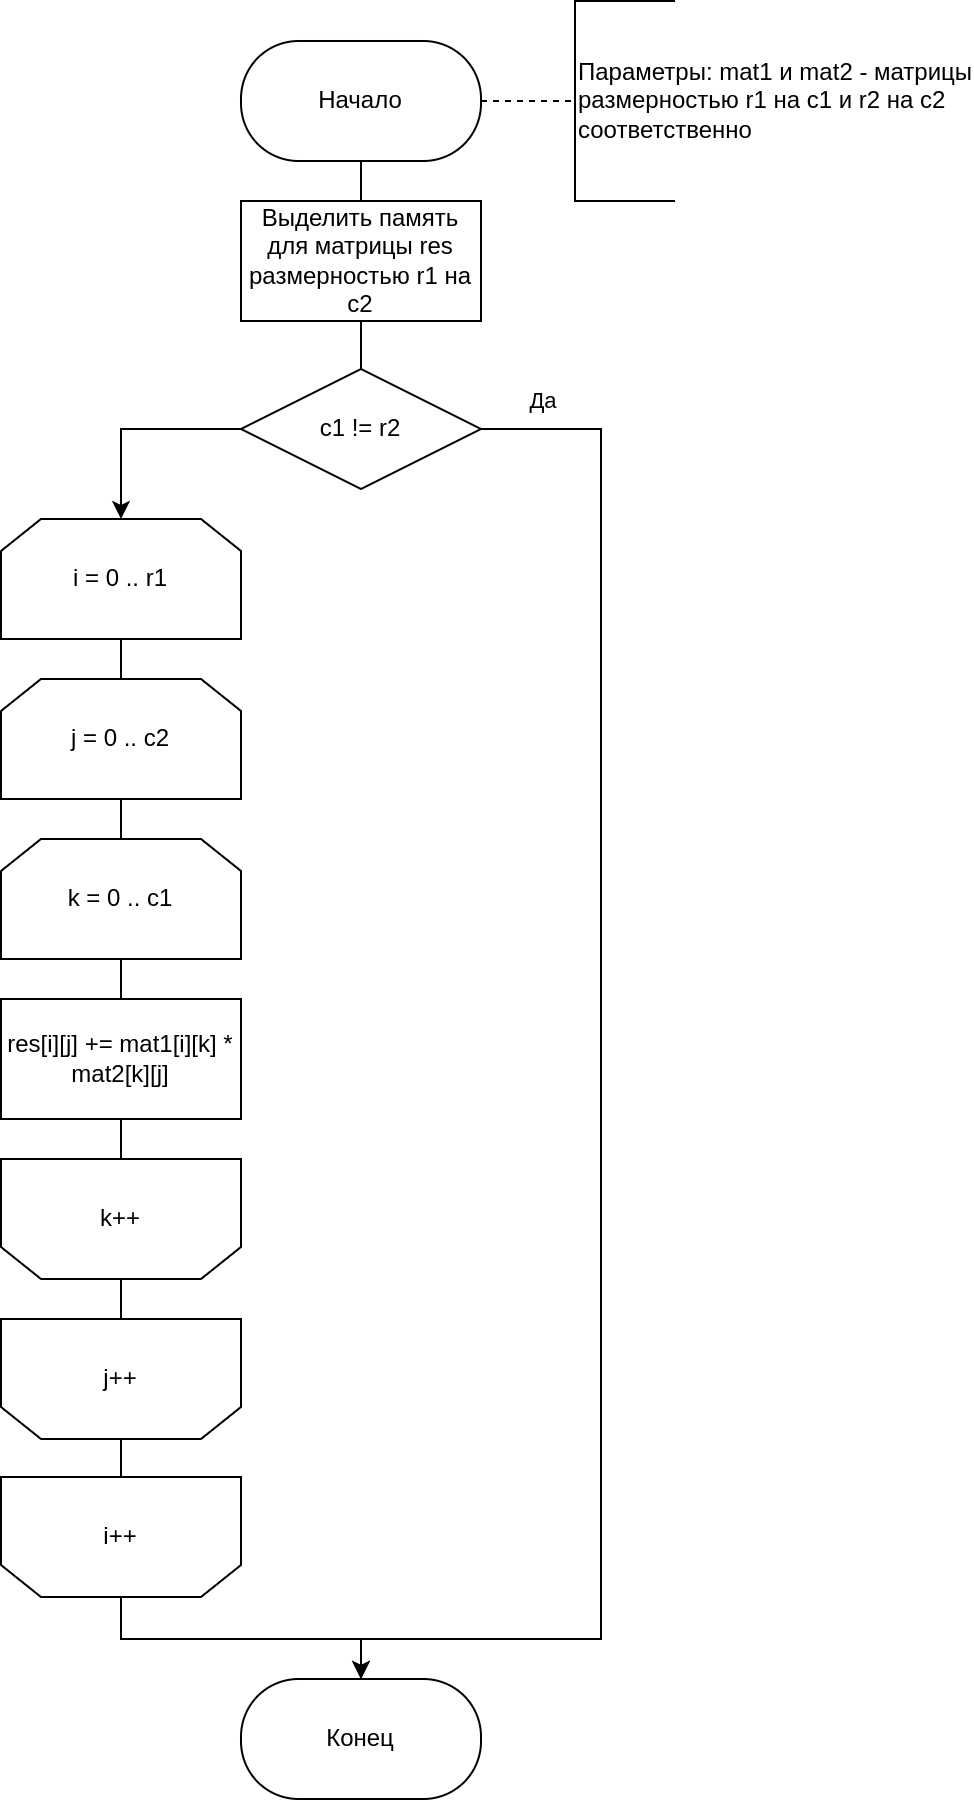
\includegraphics[scale=0.3]{img/classic.drawio.png}}
	\caption{Схема классического алгоритма умножения матриц}
\end{figure}

\section{Алгоритм Винограда для умножения матриц}

В данном алгоритме в конце необходимо сделать проверку на чётность для того, чтобы не потерять элементы при нечётных размерах матрицы.

Используемые типы и структуры данных включают в себя:
\begin{enumerate}
	\item integer, целое число - используется для хранения индексов и размерностей матрицы
	\item matrix, массив массивов вещественного типа - используется для хранения двух входных матриц и матрицы, хранящей результат умножения
\end{enumerate}

Схема алгоритма Винограда представлена на рисунке:
\begin{figure}[ph!]
	\center{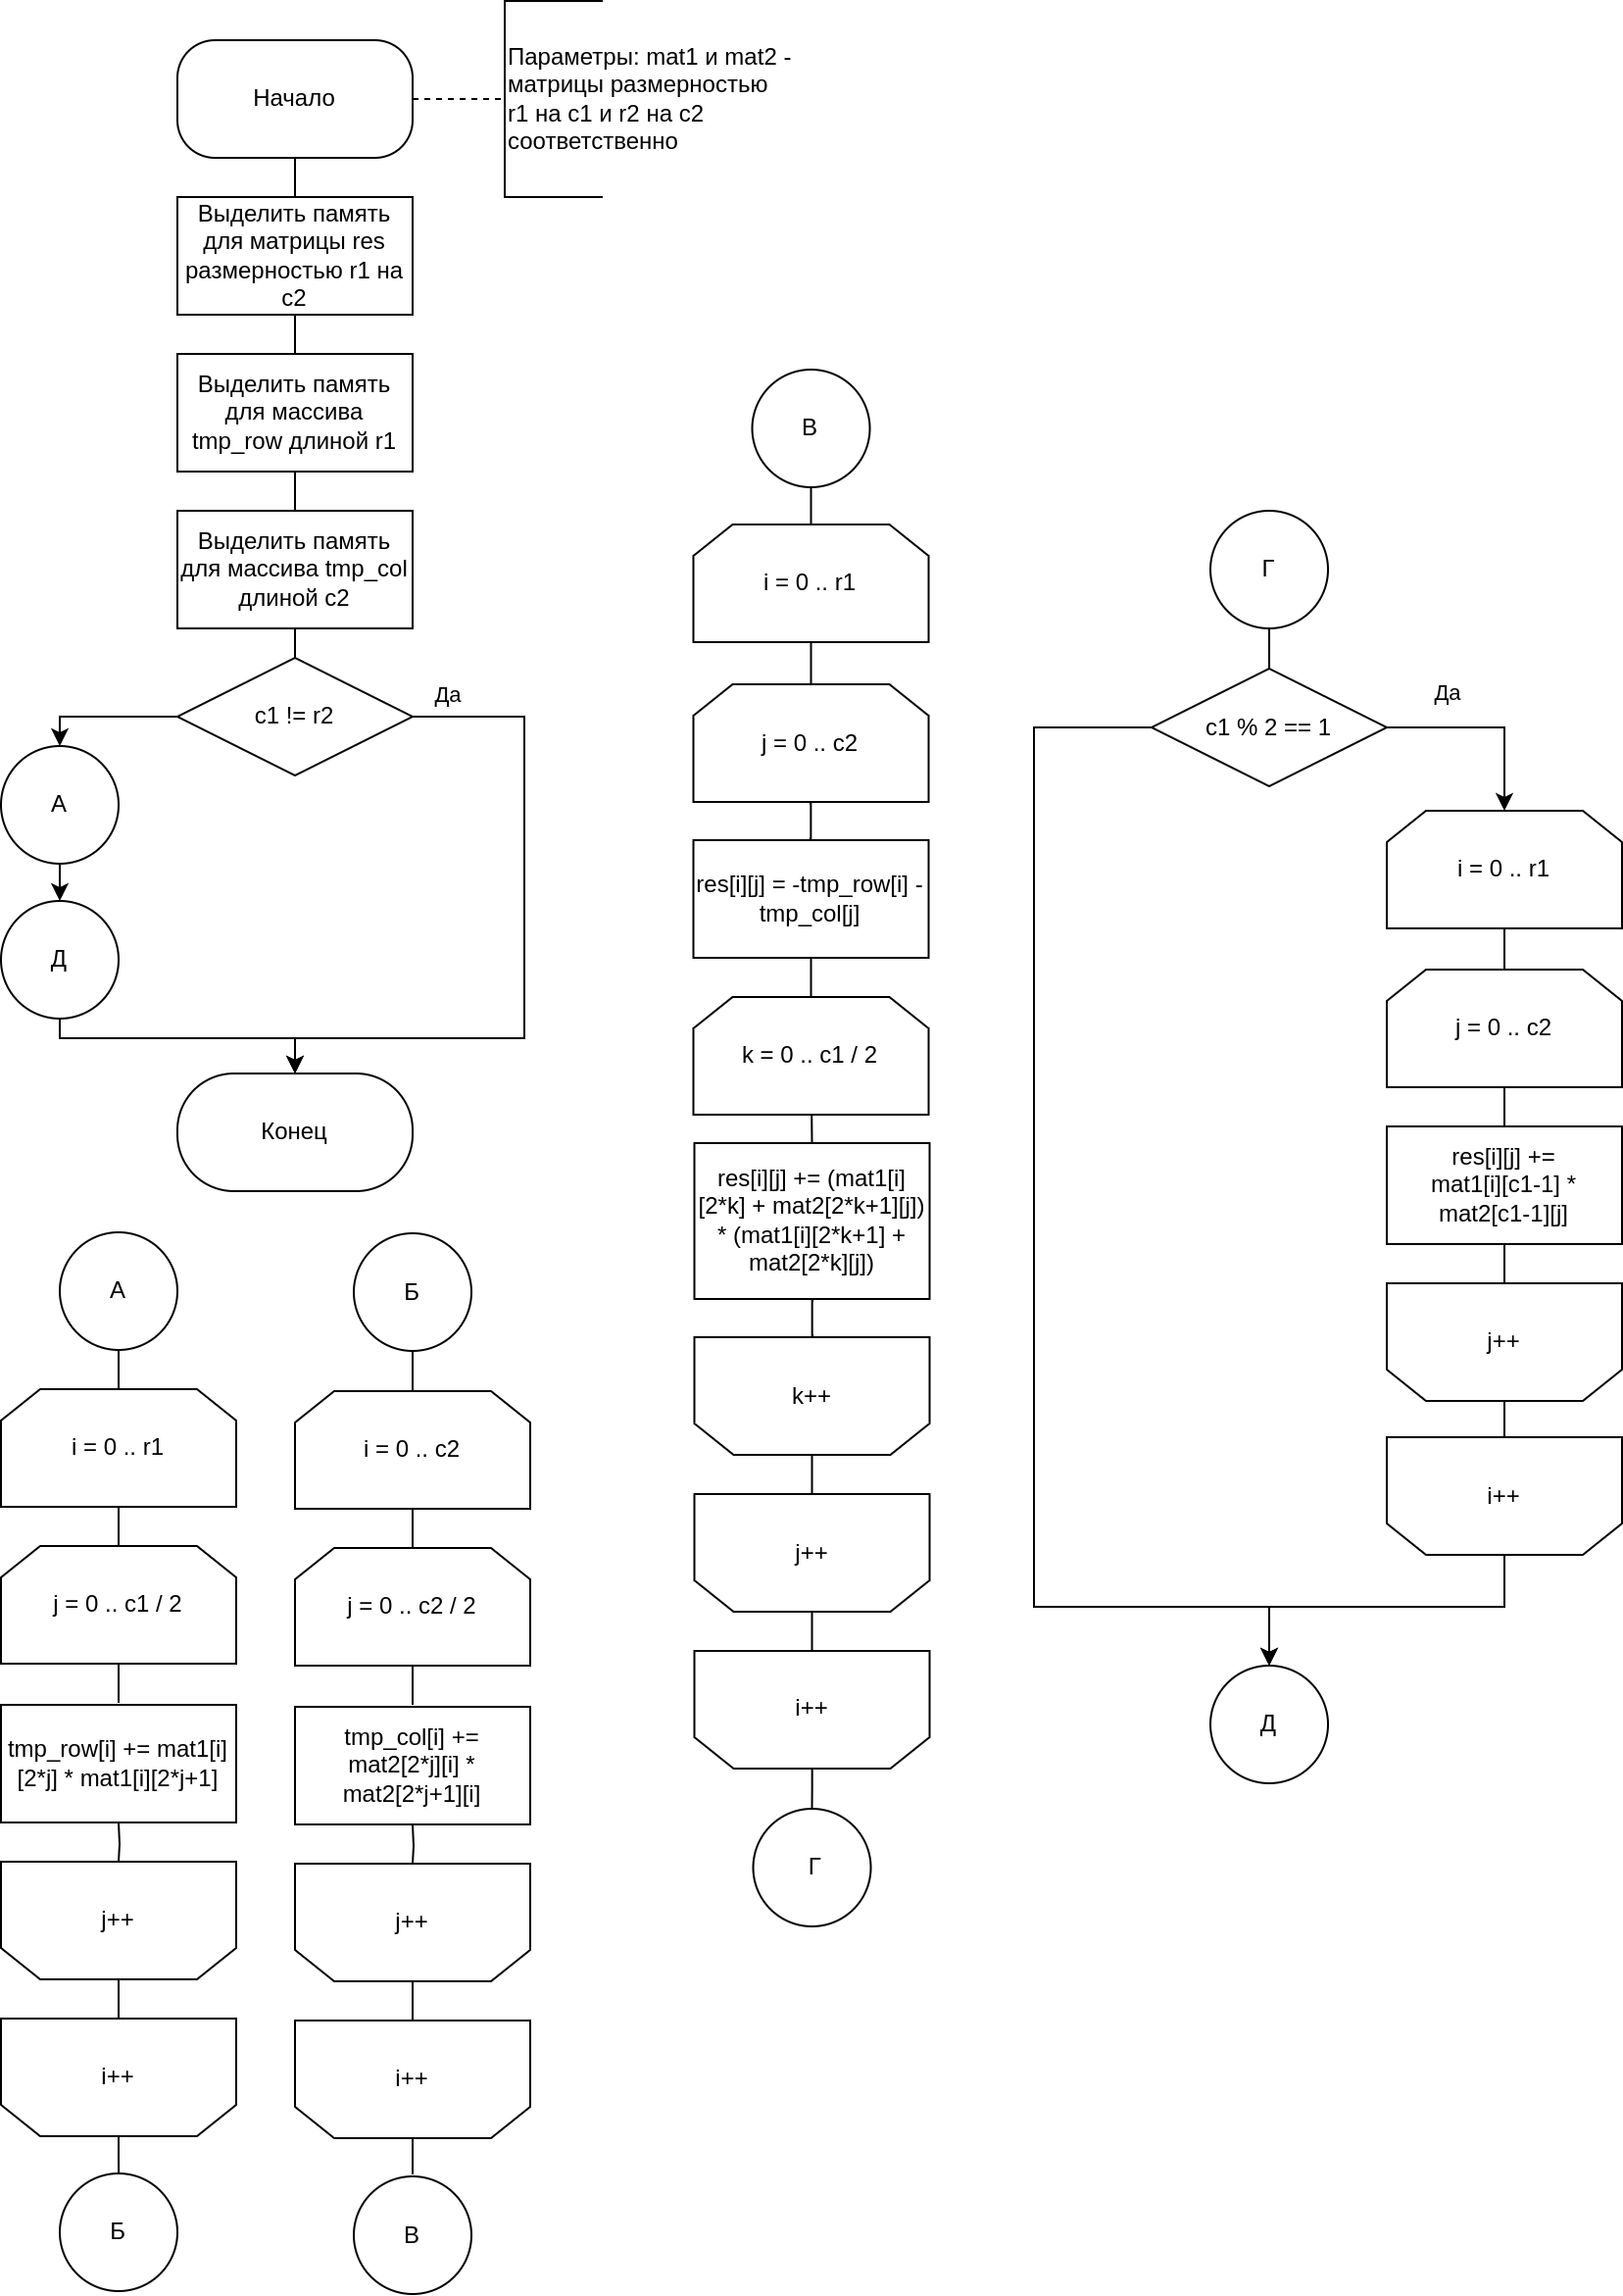
\includegraphics[scale=0.3]{img/vin.drawio.png}}
	\caption{Схема алгоритма Винограда}
\end{figure}

\section{Оптимизированный алгоритм Винограда для умножения матриц}

Для оптимизации алгоритма Винограда была добавлена операция +=, введены буферы, позволяющие не вычислять часть выражения повторно, и использованы битовые операции, имеющие меньшую трудоёмкость, чем обычные.

Используемые типы и структуры данных включают в себя:
\begin{enumerate}
	\item integer, целое число - используется для хранения индексов и размерностей матрицы
	\item matrix, массив массивов вещественного типа - используется для хранения двух входных матриц и матрицы, хранящей результат умножения
\end{enumerate}

Схема оптимизированного алгоритма Винограда представлена на рисунке:
\begin{figure}[ph!]
	\center{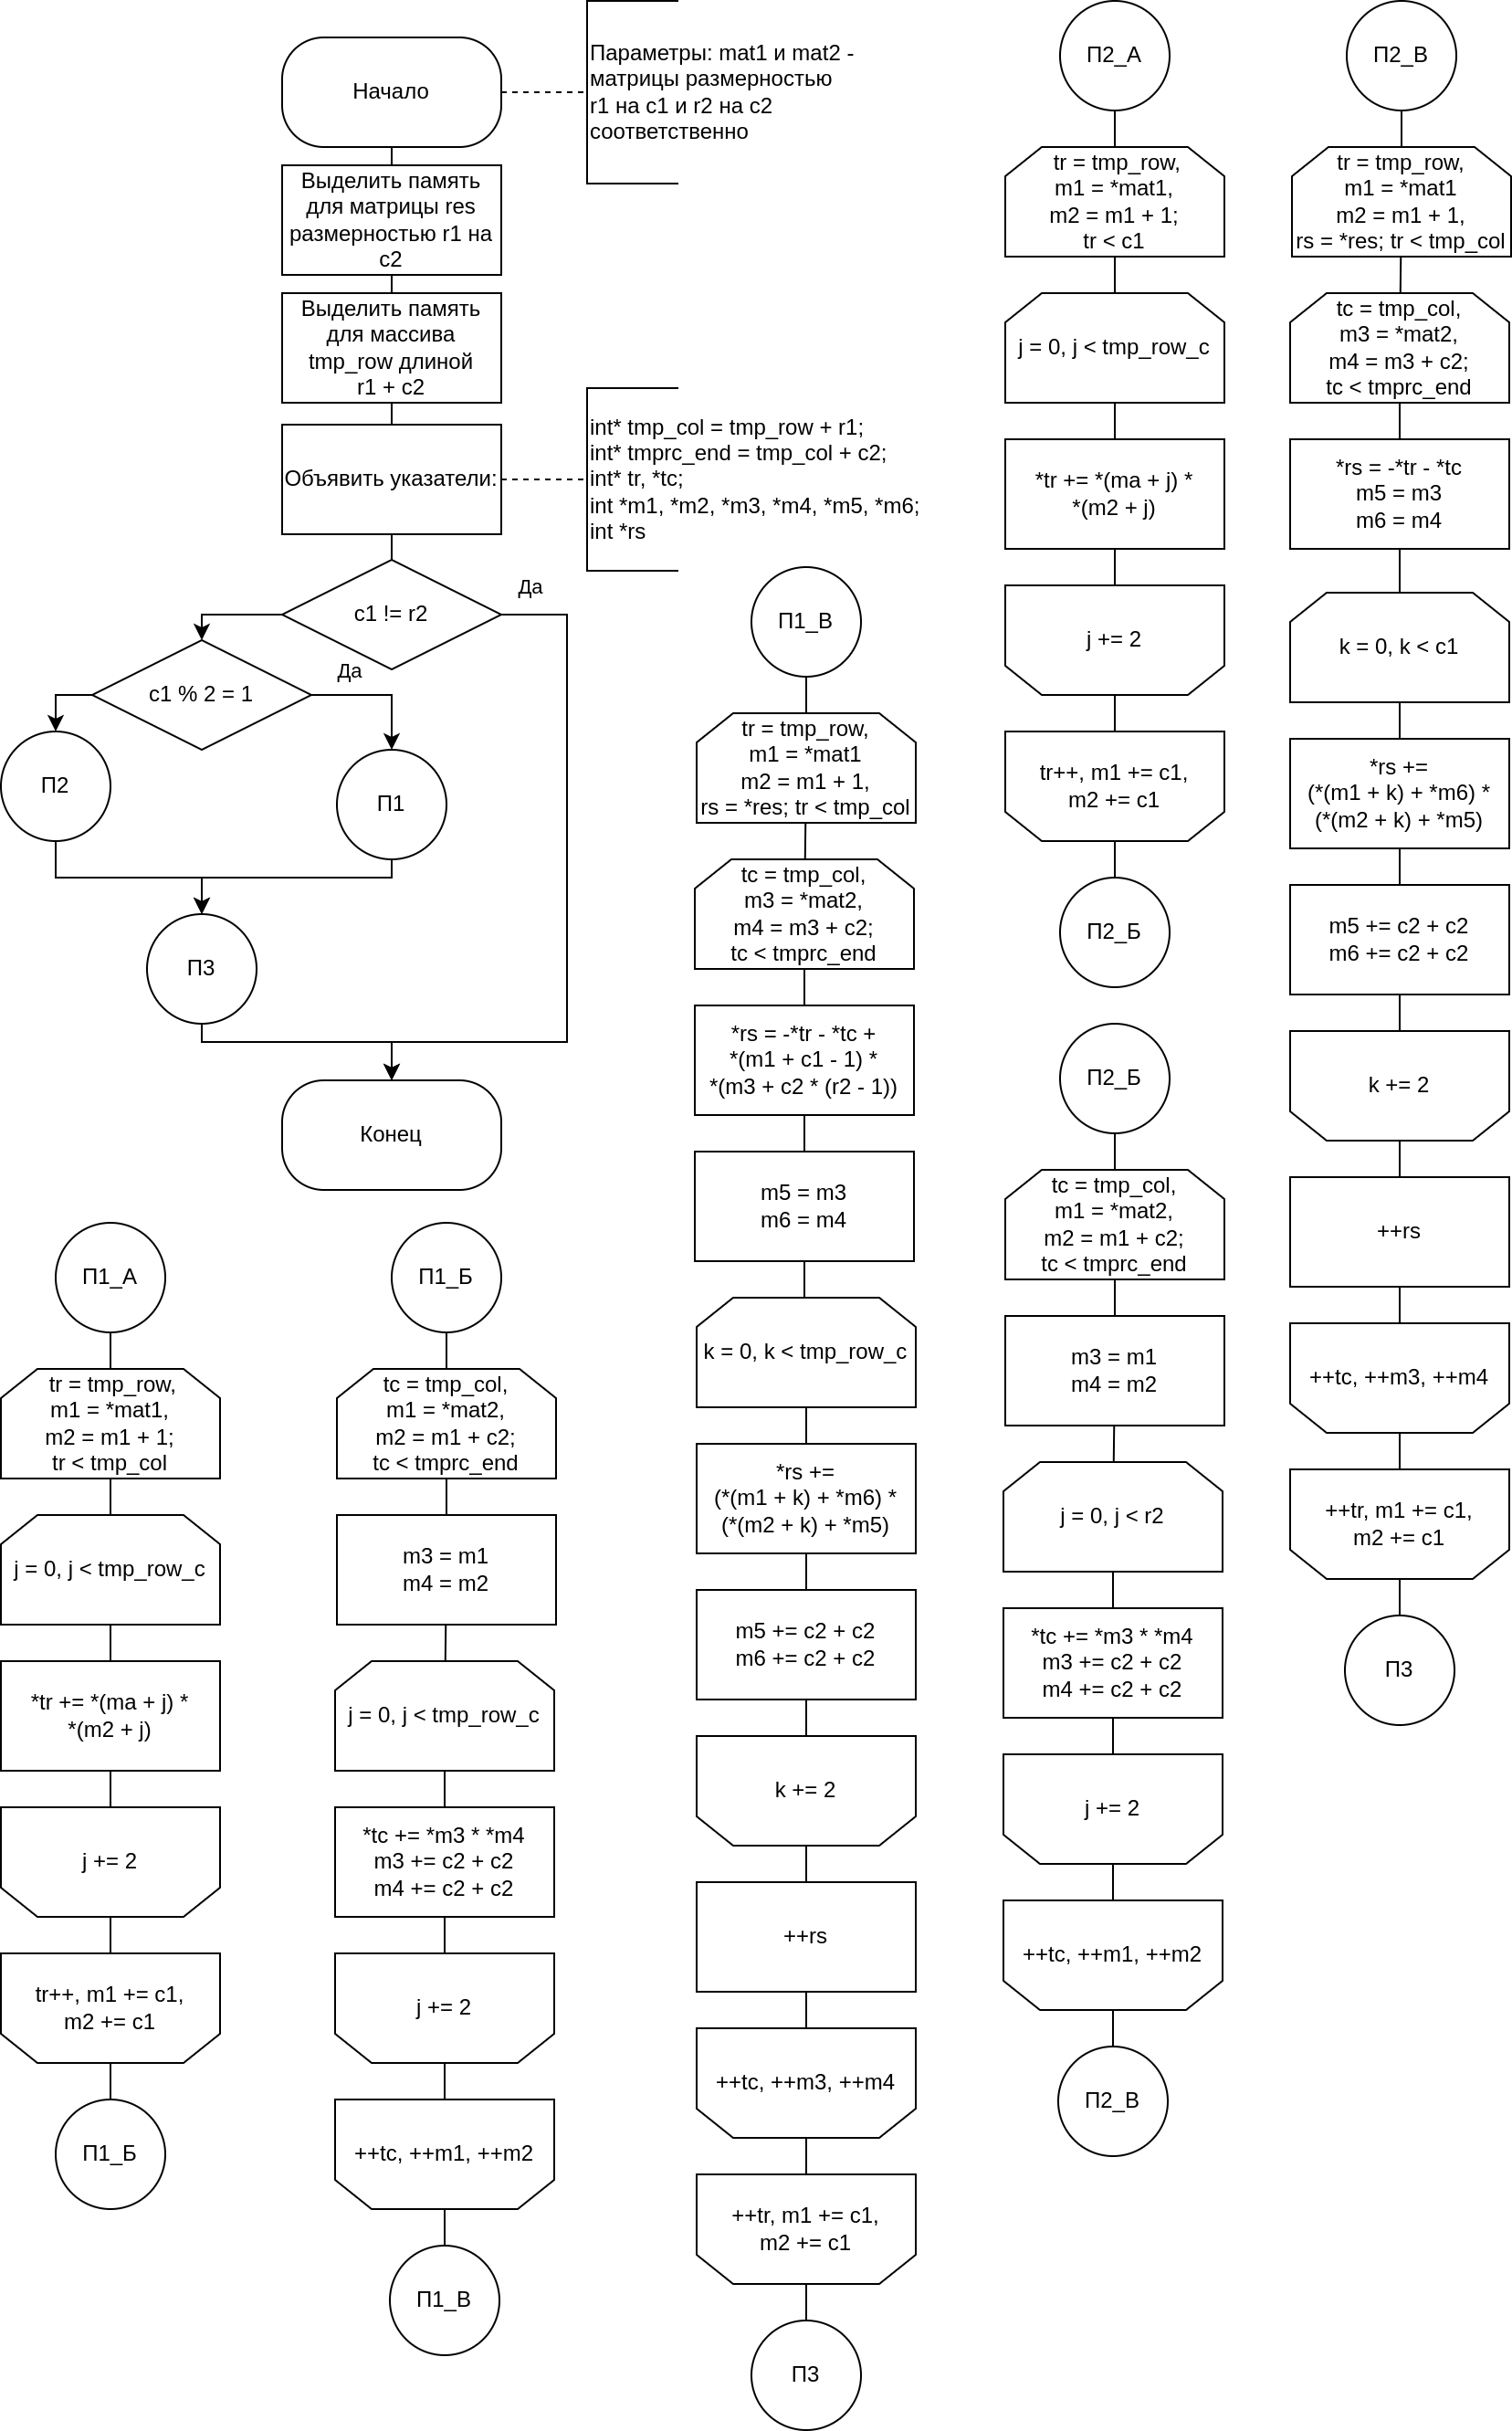
\includegraphics[scale=0.2]{img/opt_vin.drawio.png}}
	\caption{Схема оптимизированного алгоритма Винограда}
\end{figure}

\section{Трудоёмкость алгоритмов}
Проведём оценку трудоёмкости алгоритмов на основе описанной выше схемы. В приведённых ниже вычислениях констранты N, K и N - целые константы, обозначающие размеры матриц A - $N \times K$, B - $K \times M$. 

\begin{table}[h!]
  \begin{center}
    \captionsetup{justification=raggedright}
    \caption{Оценка трудоёмкости для классического алгоритма}
    \label{tab:workcost_classic}
    \begin{tabular}{c|c}
      \textbf{Трудоёмкость} & \textbf{Оценка трудоёмкости}\\
      \hline
	$F_{\text{классического}}$ & 2 + N(2 + 2 + M(2 + 2 + K(2 + $F_{\text{тела}}$)))\\
	$F_{\text{тела}}$ & 2 + 2 + 2 * 2
    \end{tabular}
  \end{center}
\end{table}
Результирующая трудоёмкость - $F_{\text{классического}}$ = (10 * N * K * M) + (4 * N * M) + (4 * N) + 2

\begin{table}[h!]
  \begin{center}
    \captionsetup{justification=raggedright}
    \caption{Оценка трудоёмкости для алгоритма Винограда}
    \label{tab:workcost_classic}
    \begin{tabular}{c|c}
      \textbf{Трудоёмкость} & \textbf{Оценка трудоёмкости}\\
      \hline
	$F_{\textbf{инициализации}}$ & 2 * 3\\
	$F_{\textbf{заполнения col\_vec}}$ & 2 + M * (2 + 2 + K / 2 * (3 + 6 + 6))\\
	$F_{\textbf{заполнения row\_vec}}$ & 2 + N * (2 + 2 + K / 2 * (3 + 6 + 6))\\
	$F_{\textbf{вычисления результата}}$ & 2 + N * (2 + 2 + M * (2 + 7 + 2 + K / 2 * (3 + 23)))\\
	$F_{\textbf{условия нечётности}}$ & 2\\
	$F_{\textbf{учёта нечётных матриц}}$ & 2 + N *(2 + 2 + M * (2 + 8 + 5))
    \end{tabular}
  \end{center}
\end{table}
Результирующая трудоёмкость - $F_{\text{Винограда}}$ = 13 * M * N * K + 7.5 * K * N + 7.5 * K * M + 11 * M * N + 8 * N + 4 * M + 14 + 
$\left[ 
  \begin{array}{c}
    0 \\
    15 ∗ M ∗ N + 4 ∗ N + 2 \\
  \end{array}
\right.$


\begin{table}[h!]
  \begin{center}
    \captionsetup{justification=raggedright}
    \caption{Оценка трудоёмкости для оптимизированного алгоритма Винограда}
    \label{tab:workcost_classic}
    \begin{tabular}{c|c}
      \textbf{Трудоёмкость} & \textbf{Оценка трудоёмкости}\\
      \hline
	$F_{\textbf{инициализации}}$ & 2 * 3 + 3\\
	$F_{\textbf{заполнения col\_vec}}$ & 2 + M * (2 + 2 + K / 2 * (3 + 6 + 6))\\
	$F_{\textbf{заполнения row\_vec}}$ & 2 + N * (2 + 2 + K / 2 * (3 + 6 + 6))\\
	$F_{\textbf{вычисления результата}}$ &2 + N * (2 + 2 + M * (2 + 5 + 3 + 2 + K / 2 * (2 + 14)))\\
	$F_{\textbf{условия нечётности}}$ & 2\\
	$F_{\textbf{учёта нечётных матриц}}$ & 2 + 2 + N * (2 + 2 + M * (2 + 6 + 2))
    \end{tabular}
  \end{center}
\end{table}
Результирующая трудоёмкость - $F_{\text{Винограда оптимизированного}}$ = 8 * M * N * K + 5 * K * N + 5 * K * M + 12 * M * N
+ 8 * N + 4 * M + 17 +
$\left[ 
  \begin{array}{c}
    0 \\
    10 ∗ M ∗ N + 4 ∗ N + 4 \\
  \end{array}
\right.$
\newpage

\section{Функциональная схема ПО}
На изображении ниже представлена функиональная схема разрабатываемого ПО. На вход подаются две матрицы и их размерности и при помощи алгоритмов, реализованных на языке Python мы получаем в результате работы новую матрицу, содерждащую в себе результат операции.

\newpage

\begin{figure}[ph!]
	\center{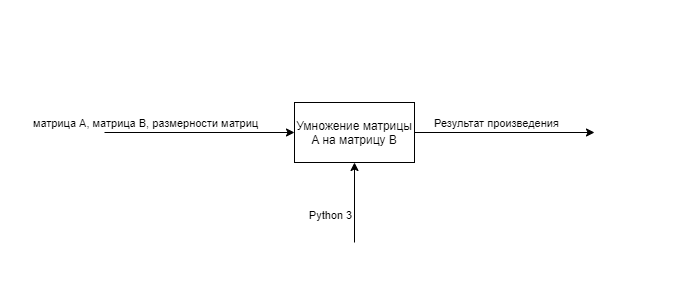
\includegraphics[scale=1.0]{idef_0}}
	\caption{IDEF0 диаграмма разрабатываемой программы}
\end{figure}

\section{Вывод}
В данном разделе были рассмотрены схемы алгоритмов для каждого из способов вычисления произведения матриц, и были определены тесты для каждого алгоритма, были описаны типы и структуры данных, использующихся в алгоритмах. Также была произведена оценка трудоёмкости для изучаемых алгоритмов и приведена функциональная схема разрабатываемого ПО.

\chapter{Технологический раздел}

В данном разделе будут рассмотрены подробности реализации описаных выше алгоритмов. Также будут обоснованы выбор языка программирования для реализации, выбор библиотек для проведения экспериментов и представлены важные фрагменты кода написанной в рамках работы программы.

\section{Выбор языка программирования}

В качестве языка программирования для реализации данной лабораторной работы использовался язык программирования python (3.9.7) [1] в целях упрощения работы со структурами данных и визцализацией данных сравнительных анализов и наличием опыта работы с данным языком программирования. В качестве среды разработки использовалась Visual Studio Code [2]. 

\section{Сведения о модулях программы}

Реализованное ПО состоит из трёх модулей:
\begin{enumerate}
	\item algos.py - в данном модуле реализованы алгоритмы умножения матриц;
	\item time.py- в данном модуле реализованы замеры временных характеристик алгоритмов;
	\item tests.py - в данном модуле реализованы тесты программ.
\end{enumerate}

\section{Реализация алгоритмов умножения матриц}

\begin{lstlisting}[label=some-code-1,caption=Реализация классического умножения матриц]
def classicMatrixMultiplation(result, mat_a, mat_b, n, k, m):
    for i in range(n):  # Iterate over rows of mat_a
        for j in range(m):  # Iterate over columns of mat_b
            result[i][j] = sum(mat_a[i][l] * mat_b[l][j] for l in range(k))  # Sum
    return result

\end{lstlisting}

\begin{lstlisting}[label=some-code-2,caption=Алгоритм Винограда для умножения матриц]
def vinogradMatrixMultiplation(result, mat_a, mat_b, n, k, m):
    row_vec = [sum(mat_a[i][j << 1] * mat_a[i][(j << 1) + 1] for j in range(k >> 1)) for i in range(n)]
    col_vec = [sum(mat_b[j << 1][i] * mat_b[(j << 1) + 1][i] for j in range(k >> 1)) for i in range(m)]

    for i in range(n):
        for j in range(m):
            result[i][j] = -row_vec[i] - col_vec[j]
            for l in range(k >> 1):  # binary instead of multiplication
                result[i][j] += (mat_a[i][(l << 1) + 1] + mat_b[l << 1][j]) * (mat_a[i][l << 1] + mat_b[(l << 1) + 1][j])

    if k % 2 == 1:
        for i in range(n):
            for j in range(m):
                result[i][j] += mat_a[i][k - 1] * mat_b[k - 1][j]

    return result
\end{lstlisting}

\begin{lstlisting}[label=some-code-3,caption=Оптимизированный алгоритм Винограда для умножения матриц]
def vinogradMatrixOptimized(result, mat_a, mat_b, n, k, m):
    
    row_vec = [0] * n
    col_vec = [0] * m

    for i in range(n):
        for j in range(0, k - (k % 2), 2):
            row_vec[i] += mat_a[i][j] * mat_a[i][j + 1]

    for i in range(m):
        for j in range(0, k - (k % 2), 2):
            col_vec[i] += mat_b[j][i] * mat_b[j + 1][i]

    
    k_mod = k - (k % 2)
    for i in range(n):
        for j in range(m):
            temp = -row_vec[i] - col_vec[j]
            for l in range(0, k_mod, 2):
                temp += (mat_a[i][l + 1] + mat_b[l][j]) * (mat_a[i][l] + mat_b[l + 1][j])
            result[i][j] = temp

    
    if k % 2 == 1:
        for i in range(n):
            for j in range(m):
                result[i][j] += mat_a[i][k - 1] * mat_b[k - 1][j]

    return result


\end{lstlisting}

\section{Реализация тестирования алгоритмов}

Для тестирования алгоритмов было реализованы следующие тесты:
\begin{enumerate}
	\item тест на двух матрицах размером n x k и k x m, где n > 0, k >  0, m > 0;
	\item тест на двух матрицах размером n x k и k x m, где n = 1, k >  0, m > 0;
	\item тест на двух матрицах размером n x k и k x m, где n > 0, k >  0, m = 1;
	\item тест на двух матрицах размером n x k и k x m, где n > 0, k >  0, m > 0, и первая матрица - нулевая;
	\item тест на двух матрицах размером n x k и k x m, где n > 0, k >  0, m > 0, и первая матрица - единичная.
\end{enumerate}

\begin{lstlisting}[label=some-code-5,caption=Реализация функции рандомной генерации матриц]

def generateMatrix(n, k, m):
    a = [[rd.randint(-100, 100) for _ in range(k)] for _ in range(n)]  # Matrix a (n x k)
    b = [[rd.randint(-100, 100) for _ in range(m)] for _ in range(k)]  # Matrix b (k x m)
    res = [[0] * m for _ in range(n)]  # Result matrix (n x m) initialized with zeros
    return a, b, res

\end{lstlisting}

\begin{lstlisting}[label=some-code-6,caption=Реализация общей функции тестирования]
def caseTest(matrix_mult_function, n, k, m):
    # Generate random matrices
    mat_a, mat_b, expected_result = generateMatrix(n, k, m)

    # Perform the matrix multiplication
    result = matrix_mult_function(expected_result, mat_a, mat_b, n, k, m)

    # Calculate the expected result using classic matrix multiplication
    expected_result = classicMatrixMultiplation([[0] * m for _ in range(n)], mat_a, mat_b, n, k, m)

    # Check if the results match
    if result == expected_result:
        print(f"Test passed for {matrix_mult_function.__name__}!")
    else:
        print(f"Test failed for {matrix_mult_function.__name__}!")
        print("Expected result:")
        printMatrix(expected_result)
        print("Actual result:")
        printMatrix(result)

\end{lstlisting}

\begin{lstlisting}[label=some-code-7,caption=Реализация функции для случая нулевой матрицы]
def testNullCase(n, k, m, case_name):
    print(case_name)
    print('Parameters: ', n, k, m)
    a = [[0 for j in range(0, k)] for i in range(0, n)]
    b = [[rd.randint(-100, 100) for j in range(0, m)] for i in range(0, k)]
    res = [[0 for j in range(0, m)] for i in range(0, n)]

    res_classic = classicMatrixMultiplation(res.copy(), a, b, n, k, m)
    res_vinograd = res.copy()
    res_vinograd_opt = res.copy()

    print('Multiply result: ')
    printMatrix(a)
    printMatrix(b)
    printMatrix(res_classic)
    printMatrix(res_vinograd)
    printMatrix(res_vinograd_opt)

    print("Checking the results: ")
    print(matrixCheck(res_classic, res_vinograd) == matrixCheck(res_classic, res_vinograd_opt) == matrixCheck(res_vinograd_opt, res_vinograd))
    print('===\n')
\end{lstlisting}

\begin{lstlisting}[label=some-code-8,caption=Реализация для случая единичной матрицы]
def testOnesCase(n, k, m, case_name):
    print(case_name)
    print('Parameters: ', n, k, m)
    a = [[rd.randint(-100, 100) for j in range(0, k)] for i in range(0, n)]
    b = [[0 for j in range(0, m)] for i in range(0, k)]
    for i in range(0, len(b)):
        b[i][i] = 1
    res = [[0 for j in range(0, m)] for i in range(0, n)]

    classicResult = classicMatrixMultiplation(res.copy(), a, b, n, k, m)
    vinogradResults = res.copy()
    vinoradOptimizedResults = res.copy()

    print('Multiply results: ')
    printMatrix(a)
    printMatrix(b)
    printMatrix(classicResult)
    printMatrix(vinogradResults)
    printMatrix(vinoradOptimizedResults)

    print("Checking the results: ")
    print(matrixCheck(classicResult, vinogradResults) == matrixCheck(classicResult, vinoradOptimizedResults) == matrixCheck(vinoradOptimizedResults, vinogradResults))
    print('===\n')     

\end{lstlisting}


\section{Вывод}
В данном разделе была представлена реализация классического умножения матриц, алгоритма Винограда и оптимизированного алгоритма Винограда. Были разработаны алгоритмы тестирования разработанных методов по методу чёрного ящика.

\chapter{Экспериментальный раздел}

В данном разделе будут измерены временные характеристики алгоритмов умножения матриц и сделаны выводы об их временной эффективности.

\begin{table}[h!]
  \begin{center}
    \captionsetup{justification=raggedright}
    \caption{Время работы классического алгоритма умножения матриц}
    \label{tab:workcost_classic}
    \begin{tabular}{c|c}
      \textbf{Размерность матрицы} & \textbf{Время умножения}\\
      \hline
	10 & 0.0\\
	25 & 0.0\\
	50 & 0.015625\\
	75 & 0.078125\\
	100 & 0.15625\\
	125 & 0.328125\\
	150 & 0.515625\\
    \end{tabular}
  \end{center}
\end{table}

\begin{table}[h!]
  \begin{center}
    \captionsetup{justification=raggedright}
    \caption{Время работы алгоритма Винограда}
    \label{tab:workcost_classic}
    \begin{tabular}{c|c}
      \textbf{Размерность матрицы} & \textbf{Время умножения}\\
      \hline
	10 & 0.0\\
	25 & 0.0\\
	50 & 0.015625\\
	75 & 0.0625\\
	100 & 0.171875\\
	125 & 0.375\\
	150 & 0.609375\\
    \end{tabular}
  \end{center}
\end{table}

\begin{table}[h!]
  \begin{center}
    \captionsetup{justification=raggedright}
    \caption{Время работы классического алгоритма оптимизированного алгоритма Винограда}
    \label{tab:workcost_classic}
    \begin{tabular}{c|c}
      \textbf{Размерность матрицы} & \textbf{Время умножения}\\
      \hline
	10 & 0.0\\
	25 & 0.015625\\
	50 & 0.015625\\
	75 & 0.0625\\
	100 & 0.125\\
	125 & 0.234375\\
	150 & 0.375\\
    \end{tabular}
  \end{center}
\end{table}

\newpage

\begin{figure}[ph!]
	\center{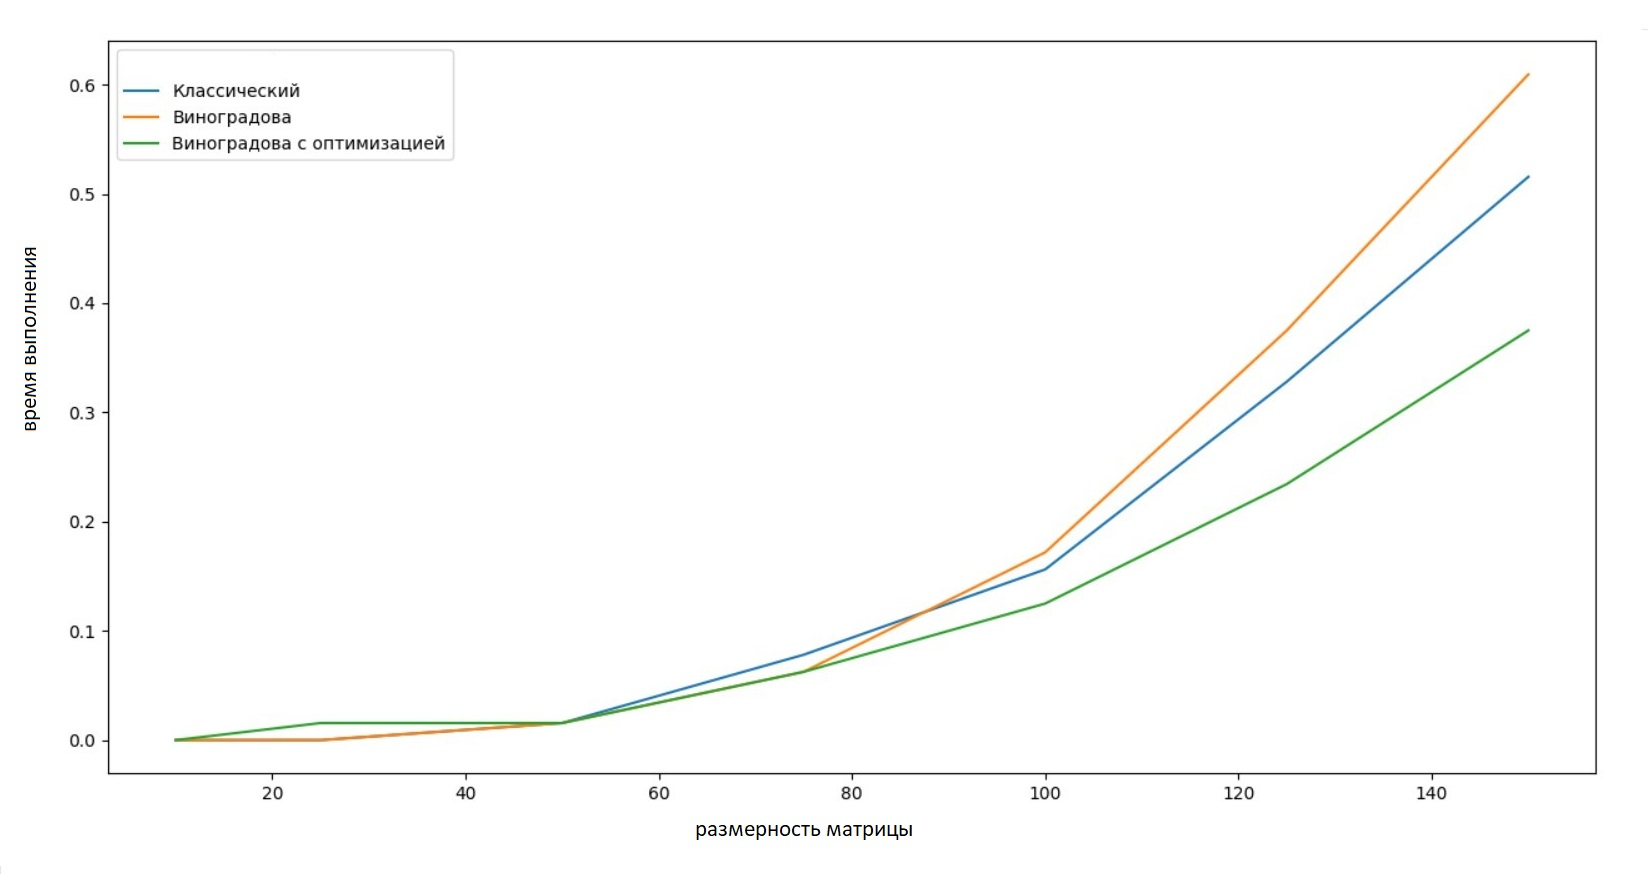
\includegraphics[scale=0.5]{res_graph}}
	\caption{График зависимости времени выполнения от размерности матрицы}
\end{figure}

\section{Вывод}
В результате экспериментов было получено, что на квадратных матрицы размерности от 10 до 80 алгоритмы работают в среднем одинаково. Однако после того, как размерность переходит 100, самым быстрым алгоритмом становится алгоритм Винограда оптимизированный, после него идёт классический алгоритм умножения матриц, и самым медленным становится алгоритм Винограда. В результате можно сделать вывод, что для матриц, размерностью больше 100 предпочтительно использовать оптимизированный алгоритм Винограда.